% =====================================================================
%  Paper 3 — RetinAI ROP staging: results compendium. IEEE two-column (IEEEtran, conference layout).
%  Build:  .venv/bin/python scripts/paper3_figures.py   (writes figs3/: figures, tab_*.tex, numbers.tex)
%          tectonic -X compile paper3_results.tex
%  Every number in this file is a macro from figs3/numbers.tex or a cell of a figs3/tab_*.tex table, both
%  generated from the files named in Table~\ref{tab:repro}; none is typed here.
%  Items in \FILL{...} must be completed by the authors before submission.
% =====================================================================
\documentclass[conference]{IEEEtran}
\usepackage{graphicx,booktabs,amsmath,amssymb,xcolor,url,array}
\graphicspath{{figs3/}}
\newcommand{\FILL}[1]{\textcolor{red}{\textbf{[FILL: #1]}}}
\IEEEoverridecommandlockouts
% Times with real bold/italic under tectonic (XeTeX); without it IEEEtran falls back to Latin Modern regular only
\usepackage{iftex}\ifXeTeX\usepackage{fontspec}\setmainfont{texgyretermes}[Extension=.otf,UprightFont=*-regular,BoldFont=*-bold,ItalicFont=*-italic,BoldItalicFont=*-bolditalic]\fi
\raggedbottom
% generated by scripts/paper3_figures.py from the files it names; do not edit
\newcommand{\selArm}{B}
\newcommand{\BcvQ}{0.825}
\newcommand{\BcvQci}{[0.737, 0.911]}
\newcommand{\BdevQ}{0.756}
\newcommand{\BdevQci}{[0.679, 0.821]}
\newcommand{\BlosoQ}{0.834}
\newcommand{\nArms}{9}
\newcommand{\nTrained}{7}
\newcommand{\poolImages}{6{,}700}
\newcommand{\poolInfants}{1{,}528}
\newcommand{\poolSources}{3}
\newcommand{\dupExcl}{14}
\newcommand{\cvScored}{6{,}686}
\newcommand{\devImages}{663}
\newcommand{\devEyes}{230}
\newcommand{\devInfants}{116}
\newcommand{\lockedImages}{661}
\newcommand{\lockedEyes}{230}
\newcommand{\nReps}{2{,}000}
\newcommand{\bootSeed}{42}
\newcommand{\cvLists}{2}
\newcommand{\devLists}{10}
\newcommand{\seedA}{42}
\newcommand{\seedB}{1337}
\newcommand{\marginCV}{0.010}
\newcommand{\marginLOSO}{0.010}
\newcommand{\nAmend}{5}
\newcommand{\lastAmendDate}{2026-10-31}
\newcommand{\protoCommit}{ac33f29}
\newcommand{\protoDate}{2026-10-20}
\newcommand{\nArch}{11}
\newcommand{\nArmsAll}{20}
\newcommand{\transArms}{F}
\newcommand{\nPairs}{12}
\newcommand{\nRuns}{10}
\newcommand{\shortcutAUC}{0.911}
\newcommand{\lockedOpened}{2026-08-18}
\newcommand{\nSevereFrom}{3}
\newcommand{\gpu}{Tesla T4}
\newcommand{\mateN}{3{,}141}
\newcommand{\mateMatched}{2{,}964}
\newcommand{\mateUnmatched}{177}
\newcommand{\mateSrcRopvl}{1{,}438}
\newcommand{\mateSrcMultiview}{896}
\newcommand{\mateSrcShenzhen}{630}
\newcommand{\mateDevTrain}{390}
\newcommand{\mateLockedTrain}{331}
\newcommand{\matePoolTrain}{1{,}647}
\newcommand{\mateTrain}{2{,}512}
\newcommand{\mateVal}{314}
\newcommand{\mateTest}{315}
\newcommand{\mateMLTest}{629}
\newcommand{\mateLeakTest}{73\%}
\newcommand{\mateLeakVal}{73\%}
\newcommand{\mateLeakMV}{99\%}
\newcommand{\mateMLFeat}{428}
\newcommand{\mateMLBest}{SVM (RBF)}
\newcommand{\mateMLAcc}{0.585}
\newcommand{\mateMLQ}{0.547}
\newcommand{\mateCNNBest}{resnest50d}
\newcommand{\mateCNNAcc}{0.835}
\newcommand{\mateCNNQ}{0.898}
\newcommand{\mateCNNEnsAcc}{0.825}
\newcommand{\mateCNNDiverged}{convnext\_tiny}
\newcommand{\mateCNNDivergedAcc}{0.530}
\newcommand{\mateFMlo}{0.787}
\newcommand{\mateFMhi}{0.832}
\newcommand{\mateFMmean}{0.814}
\newcommand{\mateFMsd}{0.023}
\newcommand{\mateFMtrainable}{6.30}
\newcommand{\mateFMtotal}{309.7}
\newcommand{\mateFMbaseAcc}{0.825}
\newcommand{\mateFMbaseTrainable}{2.37}
\newcommand{\mateFMcomboAcc}{0.651}
\newcommand{\mateEnsAcc}{0.844}
\newcommand{\mateEnsQ}{0.900}
\newcommand{\mateBestAcc}{0.860}
\newcommand{\mateBestQ}{0.908}
\newcommand{\mateBestAUC}{0.972}
\newcommand{\mateBestN}{7}
\newcommand{\mateBestAccci}{[0.820, 0.896]}
\newcommand{\mateCIkind}{infant-clustered bootstrap}
\newcommand{\mateHalfWidth}{4}
\newcommand{\mateCommit}{424ad77}
\newcommand{\nMateSeries}{33}
\newcommand{\mateDate}{2026-11-07}
\newcommand{\vtServedEyeQ}{0.839}
\newcommand{\vtServedEyeQci}{[0.768, 0.890]}
\newcommand{\vtServedEyeAcc}{0.678}
\newcommand{\vtServedEyeMF}{0.616}
\newcommand{\vtServedImgQ}{0.493}
\newcommand{\vtServedImgAcc}{0.546}
\newcommand{\vtServedImgAUC}{0.835}
\newcommand{\vtStructParams}{20{,}512{,}600}
\newcommand{\vtDropPairs}{6{,}058}

\renewcommand{\arraystretch}{1.05}
% a results compendium is mostly floats: let pages carry several, full-width ones included
\setcounter{topnumber}{4}\setcounter{dbltopnumber}{4}\setcounter{totalnumber}{10}
\renewcommand{\topfraction}{0.95}\renewcommand{\dbltopfraction}{0.95}\renewcommand{\textfraction}{0.05}
\renewcommand{\floatpagefraction}{0.8}\renewcommand{\dblfloatpagefraction}{0.8}

\title{RetinAI ROP Staging: A Results Compendium of Every Model Trained (2026)}

\author{\IEEEauthorblockN{Praharsh Nagpure, \FILL{R. Bait full name}, \FILL{P. Rangnekar full name},\\ \FILL{Y. Shengale full name}, and \FILL{A. Kumar full name}}
\IEEEauthorblockA{Department of Automation and Robotics, Vivekanand Education Society's Institute of Technology, Mumbai, India\\
Corresponding author: \FILL{name, e-mail, ORCID}}}

\begin{document}
\maketitle

\begin{abstract}
This document reports, without discussion, every model the RetinAI project trained for staging retinopathy of prematurity (ROP) in 2026, the protocol each was scored under, and the file each number comes from. The current generation (\nArms{} arms, A--I) shares one pre-registered protocol: patient-grouped five-fold cross-validation (CV) on \poolImages{} photographs of \poolInfants{} infants from \poolSources{} hospitals, eye-level scoring at a fourth hospital unseen in training, and leave-one-source-out folds. The selected model, B (DINOv2 ViT-S/14), scores CV QWK5 \BcvQ{} \BcvQci{} and, at the unseen hospital, eye-level QWK5 \BdevQ{} \BdevQci{}. Earlier generations are tabulated separately under their own protocols, as are three independent packages a team member trained in November 2026 on a photo-level split of \mateN{} of the same photographs (hand-made features with classical learners, ImageNet CNNs, and a RETFound-DINOv2 adapter model; best four-class test accuracy \mateBestAcc{}), with the reasons their numbers are not comparable.
\end{abstract}

\begin{IEEEkeywords}
retinopathy of prematurity, ICROP-3, staging, benchmark, results, pre-registration
\end{IEEEkeywords}

\section{How to Read}
\textbf{Settings.} (i)~\emph{CV per photograph}: five patient-grouped folds, out-of-fold, seeds \seedA{} and \seedB{} pooled, \dupExcl{} duplicates excluded. (ii)~\emph{Unseen hospital per eye}: Multi-View development half (\devImages{} photographs, \devEyes{} eyes); eye = most severe predicted stage; descriptive; locked half unopened for A--I. (iii)~\emph{LOSO}: train on two sources, score the third.
\textbf{Metrics.} QWK5: quadratic-weighted kappa, five ordinal levels, AP-ROP folded onto stage~4/5~\cite{icrop3}; mF1: mean per-class F1, present classes; Acc.: exact six-class matches; CIs: 95\% percentile bootstrap, \nReps{} infant resamples.
\textbf{Pre-registration.} \path{PROTOCOL_V2.md} (\texttt{\protoCommit}, \protoDate{}; \nAmend{} amendments to \lastAmendDate{}); selection on CV only.
\textbf{Caveats} (\path{MODEL_HISTORY.md}): QWK definitions, eye rules and test halves changed across generations; the June binary numbers carry a device shortcut. Sections~\ref{sec:hist} and~\ref{sec:mate} are never pooled with A--I. Table~\ref{tab:best} lists every generation's best model under its own protocol with the reason it is or is not comparable.

\begin{table*}[!t]
\caption{Every generation at a glance: the best model of each under its own protocol. Only one row is the project's selected model; every other row is listed with the reason its number cannot be read against it. Teammate rows: four classes, photo-level split, test n\,=\,\mateTest{} (\mateMLTest{} for rop\_ml); CI: 95\% Wilson.}
\label{tab:best}
\centering\scriptsize\setlength{\tabcolsep}{4pt}
\begin{tabular}{@{}>{\raggedright\arraybackslash}p{1.55cm}>{\raggedright\arraybackslash}p{4.1cm}>{\raggedright\arraybackslash}p{3.0cm}>{\raggedright\arraybackslash}p{3.55cm}>{\raggedright\arraybackslash}p{4.9cm}@{}}
\toprule
Generation & Best model & Task; split; unit & Headline, own protocol & Comparable with B?\\
\midrule
v1, Jun 2026 & EfficientNet-B3, one model for ROP and DR & ROP yes/no; image-level split; photo & test acc.\ 0.733, ROP F1 0.706 & No: image-level split; other task (Table~\ref{tab:v1}) \\
Jun 2026 sweep & ResNet50 & ROP yes/no; Ostrava; photo & test AUC 0.927, QWK$_2$ 0.688 & No: device shortcut, AUC 0.911 from image size alone (Table~\ref{tab:sweep}) \\
v2, Aug 2026 & EfficientNetV2-S, structured head & 6 classes; patient-grouped 5-fold CV; photo / eye & CV QWK$_6$ 0.761; locked eye QWK5$_d$ 0.813 (seed 42) & No: own QWK definitions and checkpoint rule; re-scored as arm C (Table~\ref{tab:v2}) \\
v3/v4, Oct 2026 & \textbf{B: DINOv2 ViT-S/14, 5-fold ensemble (selected)} & 6 classes; protocol v2; photo / eye & CV QWK5 0.825 [0.737, 0.911]; unseen-hospital eye QWK5 0.756 [0.679, 0.821] & Reference (Table~\ref{tab:headline}); the served model \\
Teammate, Nov 2026 & rop\_ml: SVM (RBF) on 428 hand-made features & 4 classes; photo-level 80/20; photo & test acc.\ 0.585, QWK 0.547 & No: photo-level split (73\% of test photos share an infant with training); trained on 390 dev-half and 331 locked-half photos; four classes (Table~\ref{tab:mateml}) \\
 & rop\_cnn: resnest50d & 4 classes; photo-level 80/10/10; photo & test acc.\ 0.835, QWK 0.898 & As above (Table~\ref{tab:matecnn}) \\
 & rop\_foundation: RETFound-DINOv2 ViT-L/14 + LoRA, 3 seeds averaged & 4 classes; photo-level 80/10/10; photo & test acc.\ 0.844, QWK 0.900 & As above (Table~\ref{tab:matefm}) \\
 & \textbf{Best of the packages: 3 seeds + 4 CNNs averaged} & 4 classes; photo-level 80/10/10; photo & test acc.\ 0.860 [0.820, 0.896], QWK 0.908, AUC 0.972 & As above; selected on validation, 314 photos (Table~\ref{tab:matefm}) \\
\bottomrule
\end{tabular}

\end{table*}

\section{Current Generation (Protocol v2, Arms A--I)}
Tables~\ref{tab:headline}--\ref{tab:secondary} and Figs.~\ref{fig:selection}--\ref{fig:training}. Arms: A RETFound-Green~\cite{engelmann2025}, B DINOv2~\cite{oquab2024}, C EfficientNetV2-S~\cite{tan2021} from~\cite{nagpure2026}, D--I variants of B (Table~\ref{tab:recipe}).

\begin{table*}[!t]
\caption{Headline results, all arms, both seeds pooled. CV: pooled out-of-fold, per photograph. Dev: unseen hospital, development half, per eye. QWK5 with 95\% infant-clustered CI; Acc.\ six-class accuracy; Bal.\,acc.\ mean per-class recall; mF1 macro-F1 over present classes; AUC and AP: any ROP vs normal (mean over each arm's models). Bold letter: selected arm. $^\dagger$Transductive: saw the dev photographs unlabelled in training.}
\label{tab:headline}
\centering\scriptsize\setlength{\tabcolsep}{3pt}
\begin{tabular}{@{}ll@{\hspace{4pt}}lcccc@{\hspace{6pt}}lcccc@{}}
\toprule
 & & \multicolumn{5}{c}{CV, per photograph (6{,}686 photos)} & \multicolumn{5}{c}{Unseen hospital, dev half, per eye (230 eyes)}\\
\cmidrule(lr){3-7}\cmidrule(l){8-12}
Arm & Model & QWK5 [95\% CI] & Acc. & Bal.\,acc. & mF1 & AUC & QWK5 [95\% CI] & Acc. & mF1 & AUC & AP\\
\midrule
A & RETFound-Green ViT-S & 0.794 [0.664, 0.915] & 0.759 & 0.656 & 0.643 & 0.977 & 0.774 [0.707, 0.828] & 0.632 & 0.563 & 0.935 & 0.984 \\
\textbf{B} & DINOv2 ViT-S & 0.825 [0.737, 0.911] & 0.766 & 0.674 & 0.653 & 0.979 & 0.756 [0.679, 0.821] & 0.630 & 0.566 & 0.937 & 0.984 \\
C & EfficientNetV2-S (baseline) & 0.816 [0.713, 0.916] & 0.788 & 0.672 & 0.656 & 0.967 & 0.760 [0.680, 0.822] & 0.624 & 0.573 & 0.943 & 0.986 \\
D & DINOv2 + exam-level loss & 0.797 [0.699, 0.909] & 0.803 & 0.671 & 0.661 & 0.942 & 0.746 [0.671, 0.810] & 0.609 & 0.542 & 0.935 & 0.984 \\
E & Ensemble A+B+C & 0.821 [0.708, 0.927] & 0.787 & 0.680 & 0.664 & 0.981 & 0.770 [0.697, 0.827] & 0.639 & 0.568 & 0.944 & 0.986 \\
F$^\dagger$ & DINOv2 + adaptation & 0.812 [0.704, 0.915] & 0.761 & 0.663 & 0.644 & 0.980 & 0.744 [0.665, 0.812] & 0.624 & 0.552 & 0.940 & 0.985 \\
G & DINOv2 at 518 px & 0.814 [0.706, 0.915] & 0.764 & 0.667 & 0.647 & 0.984 & 0.767 [0.697, 0.827] & 0.627 & 0.551 & 0.939 & 0.985 \\
H & DINOv2 on the v4 pool & 0.813 [0.707, 0.914] & 0.765 & 0.660 & 0.646 & 0.982 & 0.750 [0.674, 0.814] & 0.620 & 0.556 & 0.941 & 0.985 \\
I & DINOv2, v4 pool + v4 recipe & 0.821 [0.727, 0.912] & 0.750 & 0.645 & 0.618 & 0.982 & 0.776 [0.705, 0.834] & 0.633 & 0.561 & 0.944 & 0.986 \\
\bottomrule
\end{tabular}

\end{table*}

\begin{figure}[!t]
\centering
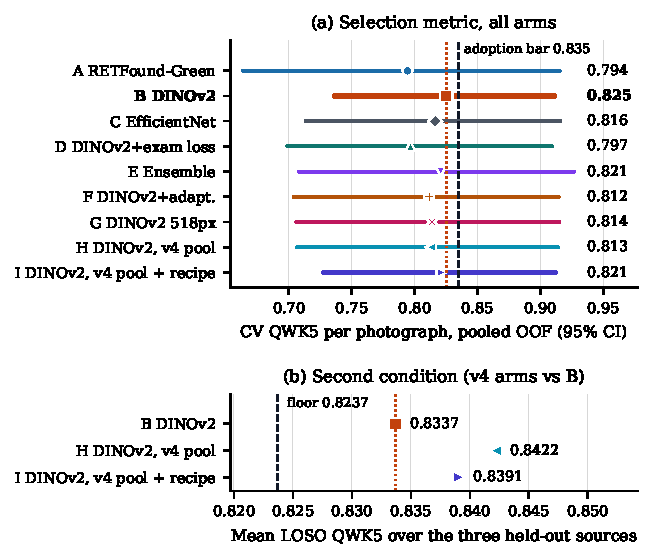
\includegraphics[width=\columnwidth]{fig_selection.pdf}
\caption{Selection. (a) CV QWK5 per photograph, pooled out-of-fold, 95\% CI. Dotted: B, chosen by the v3 rule. Dashed: the Amendment~5c adoption bar (B $+$ \marginCV{}) a v4 arm (H, I) had to reach. (b) Its second condition: mean LOSO QWK5 over three held-out sources at least B $-$ \marginLOSO{} (dashed). No v4 arm met both; \selArm{} stays.}
\label{fig:selection}
\end{figure}

\begin{figure}[!t]
\centering
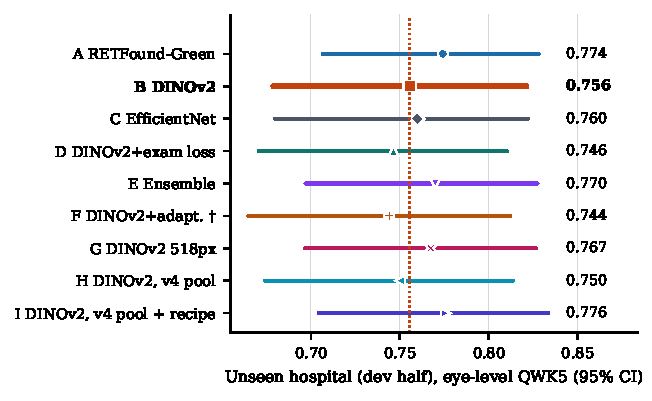
\includegraphics[width=\columnwidth]{fig_dev_eye.pdf}
\caption{Unseen hospital, development half: eye-level QWK5, 95\% CI, \devLists{} fold-seed models per arm. Descriptive; selected nothing. $^\dagger$Transductive.}
\label{fig:dev}
\end{figure}

\begin{figure}[!t]
\centering
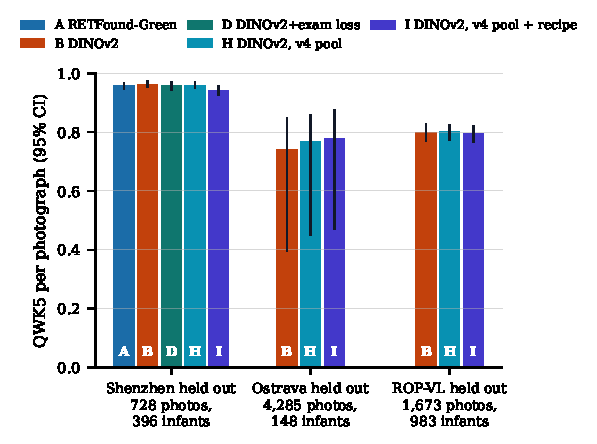
\includegraphics[width=\columnwidth]{fig_loso.pdf}
\caption{LOSO QWK5 per photograph with 95\% CI (Table~\ref{tab:loso}); bars labelled by arm. Fold compositions in Table~\ref{tab:losofolds}.}
\label{fig:loso}
\end{figure}

\begin{table*}[!t]
\caption{Recall / precision per class, both seeds pooled. Upper block: CV per photograph; lower block: unseen hospital (dev half) per eye. Class counts in each block's header. Classes~\cite{icrop3}: S stage, AP aggressive ROP.}
\label{tab:stage}
\centering\scriptsize\setlength{\tabcolsep}{4pt}
\begin{tabular}{@{}lcccccc@{}}
\toprule
Arm & Normal & Stage 1 & Stage 2 & Stage 3 & Stage 4/5 & AP-ROP\\
\midrule
\multicolumn{7}{@{}l}{\emph{CV, per photograph; n photos: Normal 3{,}837, S1 574, S2 952, S3 617, S4/5 89, AP 617}}\\
A & 0.912 / 0.947 & 0.569 / 0.293 & 0.584 / 0.541 & 0.725 / 0.848 & 0.876 / 0.741 & 0.268 / 0.760 \\
\textbf{B} & 0.909 / 0.959 & 0.583 / 0.302 & 0.561 / 0.583 & 0.722 / 0.788 & 0.882 / 0.668 & 0.389 / 0.705 \\
C & 0.951 / 0.932 & 0.497 / 0.369 & 0.604 / 0.565 & 0.724 / 0.810 & 0.876 / 0.596 & 0.382 / 0.801 \\
D & 0.993 / 0.893 & 0.475 / 0.582 & 0.488 / 0.646 & 0.712 / 0.772 & 0.865 / 0.553 & 0.490 / 0.581 \\
E & 0.943 / 0.949 & 0.551 / 0.346 & 0.620 / 0.570 & 0.729 / 0.847 & 0.910 / 0.684 & 0.328 / 0.748 \\
F$^\dagger$ & 0.911 / 0.959 & 0.570 / 0.291 & 0.562 / 0.566 & 0.722 / 0.767 & 0.888 / 0.706 & 0.327 / 0.746 \\
G & 0.914 / 0.962 & 0.607 / 0.308 & 0.567 / 0.552 & 0.720 / 0.802 & 0.893 / 0.720 & 0.302 / 0.705 \\
H & 0.924 / 0.952 & 0.570 / 0.326 & 0.557 / 0.520 & 0.725 / 0.807 & 0.876 / 0.740 & 0.306 / 0.682 \\
I & 0.909 / 0.960 & 0.490 / 0.298 & 0.568 / 0.497 & 0.741 / 0.725 & 0.893 / 0.677 & 0.269 / 0.617 \\
\midrule
\multicolumn{7}{@{}l}{\emph{Unseen hospital (dev half), per eye; n eyes: Normal 50, S1 68, S2 46, S3 59, S4/5 5, AP 2}}\\
A & 0.930 / 0.620 & 0.521 / 0.595 & 0.544 / 0.621 & 0.585 / 0.888 & 0.540 / 0.725 & 0.650 / 0.106 \\
\textbf{B} & 0.948 / 0.623 & 0.510 / 0.607 & 0.546 / 0.666 & 0.566 / 0.867 & 0.580 / 0.760 & 0.700 / 0.088 \\
C & 0.972 / 0.633 & 0.404 / 0.621 & 0.591 / 0.544 & 0.598 / 0.883 & 0.660 / 0.704 & 0.850 / 0.135 \\
D & 0.956 / 0.606 & 0.482 / 0.591 & 0.517 / 0.632 & 0.537 / 0.867 & 0.540 / 0.768 & 0.600 / 0.067 \\
E & 0.974 / 0.627 & 0.491 / 0.623 & 0.570 / 0.625 & 0.586 / 0.887 & 0.560 / 0.718 & 0.650 / 0.096 \\
F$^\dagger$ & 0.974 / 0.626 & 0.484 / 0.633 & 0.546 / 0.654 & 0.559 / 0.867 & 0.540 / 0.717 & 0.600 / 0.064 \\
G & 0.962 / 0.624 & 0.507 / 0.597 & 0.522 / 0.639 & 0.571 / 0.899 & 0.540 / 0.700 & 0.550 / 0.070 \\
H & 0.950 / 0.625 & 0.497 / 0.600 & 0.539 / 0.622 & 0.551 / 0.864 & 0.580 / 0.802 & 0.550 / 0.071 \\
I & 0.936 / 0.649 & 0.506 / 0.648 & 0.596 / 0.628 & 0.559 / 0.821 & 0.560 / 0.783 & 0.550 / 0.067 \\
\bottomrule
\end{tabular}

\end{table*}

\begin{figure*}[!t]
\centering
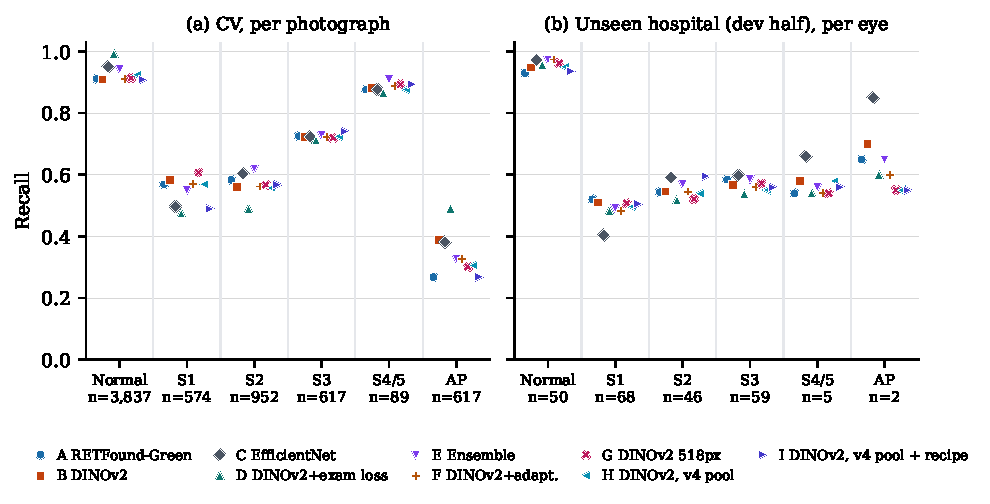
\includegraphics[width=\textwidth]{fig_stage_recall.pdf}
\caption{Recall per class, all arms: (a) CV per photograph; (b) unseen hospital per eye. n below each class: photographs (a), eyes (b). Arm identity by colour and marker.}
\label{fig:stage}
\end{figure*}

\begin{figure*}[!t]
\centering
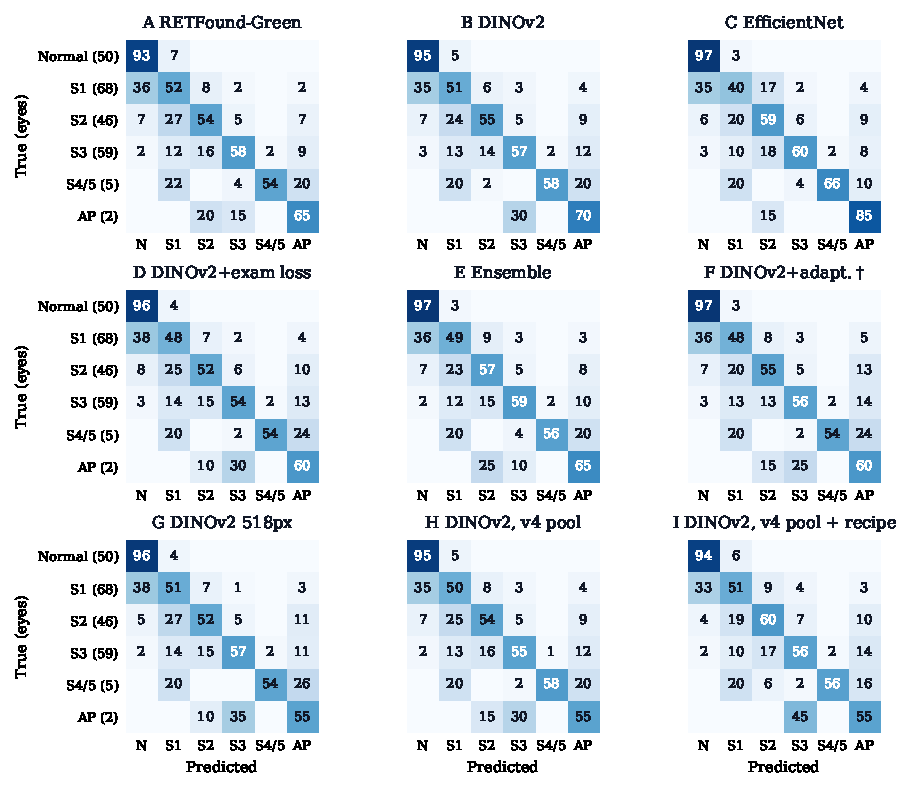
\includegraphics[width=0.8\textwidth]{fig_confusion_dev_eye.pdf}
\caption{Eye-level confusion matrices at the unseen hospital (dev half), all arms. Cell: share of the true-class row in \%, averaged over the arm's \devLists{} models (diagonal = recall); blank = 0. True-class eye counts in parentheses. N normal, S stage, AP AP-ROP. $^\dagger$Transductive.}
\label{fig:cm}
\end{figure*}

\begin{table}[!t]
\caption{CV QWK5 per photograph per fold (F0--F4) and seed, each fold scored by its own model; mean and SD over the five folds.}
\label{tab:folds}
\centering\scriptsize\setlength{\tabcolsep}{3.2pt}
\begin{tabular}{@{}ll@{\hspace{4pt}}ccccc@{\hspace{4pt}}cc@{}}
\toprule
Arm & Seed & F0 & F1 & F2 & F3 & F4 & Mean & SD\\
\midrule
A & 42 & 0.623 & 0.868 & 0.872 & 0.907 & 0.918 & 0.838 & 0.122 \\
 & 1337 & 0.595 & 0.868 & 0.882 & 0.911 & 0.916 & 0.834 & 0.135 \\
\textbf{B} & 42 & 0.743 & 0.870 & 0.853 & 0.904 & 0.898 & 0.854 & 0.065 \\
 & 1337 & 0.666 & 0.879 & 0.857 & 0.923 & 0.909 & 0.847 & 0.104 \\
C & 42 & 0.680 & 0.865 & 0.889 & 0.899 & 0.926 & 0.852 & 0.099 \\
 & 1337 & 0.667 & 0.863 & 0.853 & 0.934 & 0.917 & 0.847 & 0.106 \\
D & 42 & 0.691 & 0.851 & 0.810 & 0.897 & 0.882 & 0.826 & 0.083 \\
 & 1337 & 0.650 & 0.858 & 0.816 & 0.920 & 0.883 & 0.826 & 0.105 \\
E & 42 & 0.682 & 0.874 & 0.905 & 0.918 & 0.929 & 0.862 & 0.102 \\
 & 1337 & 0.634 & 0.881 & 0.878 & 0.933 & 0.935 & 0.852 & 0.125 \\
F$^\dagger$ & 42 & 0.673 & 0.886 & 0.841 & 0.928 & 0.878 & 0.841 & 0.099 \\
 & 1337 & 0.648 & 0.887 & 0.879 & 0.913 & 0.910 & 0.847 & 0.112 \\
G & 42 & 0.666 & 0.876 & 0.876 & 0.919 & 0.895 & 0.846 & 0.103 \\
 & 1337 & 0.646 & 0.882 & 0.875 & 0.916 & 0.915 & 0.847 & 0.114 \\
H & 42 & 0.663 & 0.880 & 0.832 & 0.915 & 0.915 & 0.841 & 0.105 \\
 & 1337 & 0.672 & 0.883 & 0.842 & 0.913 & 0.912 & 0.844 & 0.101 \\
I & 42 & 0.677 & 0.885 & 0.873 & 0.912 & 0.910 & 0.851 & 0.099 \\
 & 1337 & 0.704 & 0.877 & 0.824 & 0.915 & 0.888 & 0.841 & 0.084 \\
\bottomrule
\end{tabular}

\end{table}

\begin{table*}[!t]
\caption{Leave-one-source-out (LOSO), per photograph, seeds pooled: QWK5, mF1 and accuracy with 95\% infant-clustered CI, and mean recall per class (-- absent from the held-out source). Shenzhen is the protocol's site fold; the Ostrava and ROP-VL folds were added by Amendment~5 for B, H and I. Pool: the training pool (Table~\ref{tab:pool}).}
\label{tab:loso}
\centering\scriptsize\setlength{\tabcolsep}{3.2pt}
\begin{tabular}{@{}ll@{\hspace{4pt}}lll@{\hspace{4pt}}cccccc@{}}
\toprule
 & & & & & \multicolumn{6}{c}{Mean recall per class}\\
\cmidrule(l){6-11}
Arm & Pool & QWK5 [95\% CI] & mF1 [95\% CI] & Acc. [95\% CI] & Normal & S1 & S2 & S3 & S4/5 & AP\\
\midrule
\multicolumn{10}{@{}l}{\emph{Shenzhen held out (fold\_site.csv): 728 photos, 396 infants, 12 duplicates excluded}}\\
A & v3 & 0.958 [0.948, 0.966] & 0.832 [0.799, 0.863] & 0.867 [0.840, 0.892] & 0.99 & 0.58 & 0.79 & 0.90 & -- & -- \\
\textbf{B} & v3 & 0.962 [0.953, 0.971] & 0.841 [0.809, 0.871] & 0.882 [0.859, 0.906] & 1.00 & 0.58 & 0.81 & 0.93 & -- & -- \\
D & v3 & 0.958 [0.945, 0.968] & 0.836 [0.804, 0.867] & 0.877 [0.853, 0.900] & 1.00 & 0.53 & 0.85 & 0.90 & -- & -- \\
H & v4 & 0.960 [0.950, 0.969] & 0.839 [0.808, 0.870] & 0.877 [0.854, 0.901] & 1.00 & 0.59 & 0.79 & 0.92 & -- & -- \\
I & v4 & 0.942 [0.926, 0.956] & 0.777 [0.741, 0.814] & 0.840 [0.813, 0.868] & 1.00 & 0.39 & 0.72 & 0.92 & -- & -- \\
\midrule
\multicolumn{10}{@{}l}{\emph{Ostrava held out (fold\_loso\_ostrava.csv): 4{,}285 photos, 148 infants, 0 duplicates excluded}}\\
\textbf{B} & v3 & 0.740 [0.398, 0.845] & 0.483 [0.384, 0.596] & 0.791 [0.710, 0.868] & 0.95 & 0.14 & 0.20 & 0.36 & -- & 0.79 \\
H & v4 & 0.766 [0.452, 0.858] & 0.479 [0.380, 0.590] & 0.797 [0.718, 0.876] & 0.97 & 0.13 & 0.20 & 0.35 & -- & 0.77 \\
I & v4 & 0.779 [0.471, 0.875] & 0.487 [0.394, 0.595] & 0.804 [0.721, 0.880] & 0.97 & 0.15 & 0.19 & 0.36 & -- & 0.82 \\
\midrule
\multicolumn{10}{@{}l}{\emph{ROP-VL held out (fold\_loso\_ropvl.csv): 1{,}673 photos, 983 infants, 2 duplicates excluded}}\\
\textbf{B} & v3 & 0.800 [0.771, 0.827] & 0.452 [0.437, 0.467] & 0.677 [0.653, 0.701] & 0.94 & 0.74 & 0.60 & 0.71 & 0.00 & 0.00 \\
H & v4 & 0.801 [0.774, 0.824] & 0.443 [0.427, 0.458] & 0.658 [0.634, 0.682] & 0.89 & 0.71 & 0.60 & 0.74 & 0.00 & 0.00 \\
I & v4 & 0.796 [0.768, 0.820] & 0.462 [0.445, 0.479] & 0.676 [0.652, 0.699] & 0.94 & 0.48 & 0.67 & 0.81 & 0.00 & 0.06 \\
\midrule
\multicolumn{10}{@{}l}{\emph{Mean QWK5 over the three held-out sources (Amendment 5c): B 0.834, H 0.842, I 0.839}}\\
\bottomrule
\end{tabular}

\end{table*}

\begin{table*}[!t]
\caption{All \nPairs{} pre-specified paired contrasts (first arm minus second): QWK5 and mF1, both arms on the same infant resample, 95\% CI. CV: selection context; dev: descriptive. No row is a confirmatory test; the primary endpoint (locked-half eye-level A$-$C) is unscored.}
\label{tab:contrasts}
\centering\scriptsize\setlength{\tabcolsep}{4pt}
\begin{tabular}{@{}llllll@{}}
\toprule
 & & \multicolumn{2}{c}{CV, per photograph} & \multicolumn{2}{c}{Dev half, per eye}\\
\cmidrule(lr){3-4}\cmidrule(l){5-6}
Pair & Contrast & $\Delta$QWK5 [95\% CI] & $\Delta$mF1 [95\% CI] & $\Delta$QWK5 [95\% CI] & $\Delta$mF1 [95\% CI]\\
\midrule
A$-$C & retinal vs CNN (primary) & $-$0.022 [$-$0.052, +0.008] & $-$0.013 [$-$0.025, +0.012] & +0.014 [$-$0.012, +0.048] & $-$0.009 [$-$0.063, +0.031] \\
A$-$B & retinal vs natural & $-$0.031 [$-$0.077, +0.015] & $-$0.010 [$-$0.023, +0.036] & +0.019 [+0.000, +0.041] & $-$0.003 [$-$0.032, +0.016] \\
B$-$C & natural vs CNN & +0.009 [$-$0.018, +0.027] & $-$0.003 [$-$0.041, +0.018] & $-$0.004 [$-$0.038, +0.030] & $-$0.007 [$-$0.066, +0.042] \\
E$-$C & ensemble vs CNN & +0.005 [$-$0.007, +0.019] & +0.008 [$-$0.001, +0.024] & +0.010 [$-$0.012, +0.040] & $-$0.005 [$-$0.058, +0.034] \\
E$-$A & ensemble vs retinal & +0.026 [+0.008, +0.046] & +0.021 [+0.007, +0.029] & $-$0.004 [$-$0.020, +0.008] & +0.004 [$-$0.010, +0.022] \\
D$-$A & exam loss vs retinal & +0.002 [$-$0.057, +0.046] & +0.018 [$-$0.074, +0.055] & $-$0.028 [$-$0.048, $-$0.011] & $-$0.022 [$-$0.047, +0.019] \\
D$-$B & exam loss vs per photo & $-$0.029 [$-$0.051, +0.003] & +0.008 [$-$0.042, +0.038] & $-$0.009 [$-$0.019, +0.001] & $-$0.024 [$-$0.042, $-$0.002] \\
F$-$B & adaptation & $-$0.014 [$-$0.035, +0.008] & $-$0.009 [$-$0.021, +0.021] & $-$0.012 [$-$0.022, $-$0.002] & $-$0.014 [$-$0.027, +0.006] \\
G$-$B & 518 vs 392 px & $-$0.011 [$-$0.036, +0.012] & $-$0.006 [$-$0.020, +0.026] & +0.012 [$-$0.006, +0.032] & $-$0.014 [$-$0.037, +0.016] \\
H$-$B & v4 pool & $-$0.013 [$-$0.031, +0.009] & $-$0.007 [$-$0.017, +0.019] & $-$0.006 [$-$0.015, +0.003] & $-$0.010 [$-$0.023, +0.010] \\
I$-$B & v4 pool + recipe & $-$0.004 [$-$0.015, +0.007] & $-$0.035 [$-$0.053, $-$0.001] & +0.020 [+0.003, +0.041] & $-$0.005 [$-$0.057, +0.033] \\
I$-$H & v4 recipe & +0.009 [$-$0.007, +0.020] & $-$0.028 [$-$0.043, $-$0.010] & +0.026 [+0.006, +0.046] & +0.004 [$-$0.050, +0.045] \\
\bottomrule
\end{tabular}

\end{table*}

\begin{figure*}[!t]
\centering
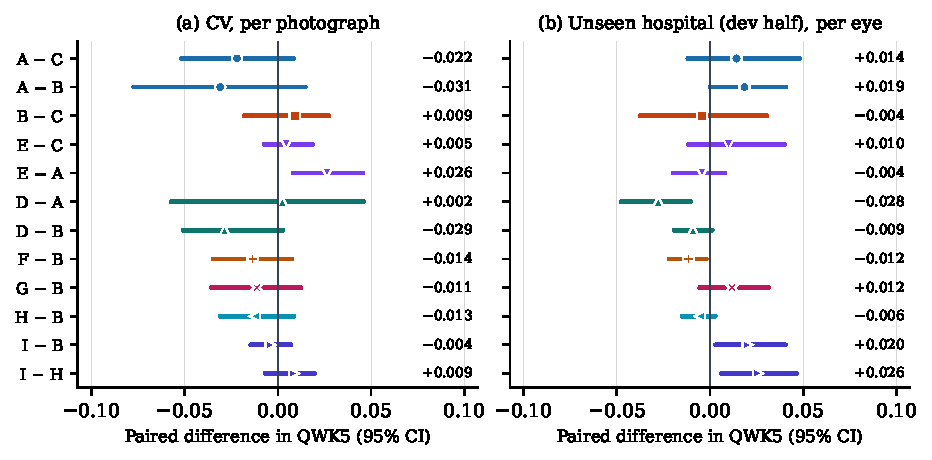
\includegraphics[width=\textwidth]{fig_contrasts.pdf}
\caption{Paired contrasts in QWK5 with 95\% CI (Table~\ref{tab:contrasts}): (a) CV, \cvScored{} photographs; (b) dev half, \devEyes{} eyes. A line crossing zero is a tie; point differences at right.}
\label{fig:contrasts}
\end{figure*}

\begin{table*}[!t]
\caption{Operating point and calibration, per arm and seed. Threshold: the largest value of the unit any-ROP score, $\max_i(1-p_{i,\mathrm{normal}})$, that keeps CV unit-level any-ROP sensitivity at or above 0.90; carried unchanged to the dev half, where sensitivity and specificity are means over the seed's five fold models. Severe: stage~\nSevereFrom{} or worse, including AP-ROP, at the same threshold. $T$: temperature fitted on CV out-of-fold unit vectors. ECE: ten bins, dev eyes, seeds pooled, as trained and after $T$ (Fig.~\ref{fig:reliability}).}
\label{tab:operating}
\centering\scriptsize\setlength{\tabcolsep}{3.4pt}
\begin{tabular}{@{}llc@{\hspace{5pt}}cccc@{\hspace{5pt}}cccc@{\hspace{5pt}}ccc@{}}
\toprule
 & & & \multicolumn{4}{c}{Any ROP vs normal} & \multicolumn{4}{c}{Severe (S3+) vs rest} & & \multicolumn{2}{c}{Dev-eye ECE}\\
\cmidrule(lr){4-7}\cmidrule(lr){8-11}\cmidrule(l){13-14}
Arm & Seed & Threshold & CV sens & CV spec & Dev sens & Dev spec & CV sens & CV spec & Dev sens & Dev spec & $T$ & as trained & with $T$\\
\midrule
A & 42 & 0.9884 & 0.900 & 0.999 & 0.650 & 1.000 & 0.952 & 0.652 & 0.924 & 0.659 & 0.840 & 0.152 & 0.205 \\
 & 1337 & 0.9887 & 0.900 & 0.996 & 0.670 & 1.000 & 0.955 & 0.651 & 0.933 & 0.640 & 0.853 &  &  \\
\textbf{B} & 42 & 0.9894 & 0.900 & 0.996 & 0.656 & 1.000 & 0.945 & 0.648 & 0.927 & 0.654 & 0.850 & 0.157 & 0.203 \\
 & 1337 & 0.9893 & 0.900 & 0.998 & 0.676 & 1.000 & 0.957 & 0.654 & 0.942 & 0.638 & 0.851 &  &  \\
C & 42 & 0.9850 & 0.900 & 0.991 & 0.680 & 1.000 & 0.948 & 0.646 & 0.894 & 0.613 & 0.917 & 0.183 & 0.208 \\
 & 1337 & 0.9805 & 0.900 & 0.993 & 0.671 & 1.000 & 0.942 & 0.645 & 0.918 & 0.633 & 0.935 &  &  \\
D & 42 & 0.9893 & 0.900 & 0.998 & 0.656 & 1.000 & 0.952 & 0.651 & 0.900 & 0.643 & 0.828 & 0.185 & 0.238 \\
 & 1337 & 0.9876 & 0.900 & 0.999 & 0.639 & 1.000 & 0.948 & 0.650 & 0.909 & 0.665 & 0.838 &  &  \\
E & 42 & 0.9866 & 0.900 & 1.000 & 0.650 & 1.000 & 0.945 & 0.650 & 0.912 & 0.654 & 0.747 & 0.135 & 0.214 \\
 & 1337 & 0.9848 & 0.900 & 0.998 & 0.662 & 1.000 & 0.941 & 0.647 & 0.918 & 0.643 & 0.762 &  &  \\
F$^\dagger$ & 42 & 0.9891 & 0.900 & 0.996 & 0.679 & 1.000 & 0.944 & 0.647 & 0.921 & 0.626 & 0.853 & 0.184 & 0.223 \\
 & 1337 & 0.9890 & 0.900 & 0.997 & 0.669 & 1.000 & 0.959 & 0.654 & 0.933 & 0.642 & 0.863 &  &  \\
G & 42 & 0.9882 & 0.900 & 0.996 & 0.643 & 1.000 & 0.949 & 0.649 & 0.921 & 0.665 & 0.854 & 0.174 & 0.210 \\
 & 1337 & 0.9897 & 0.900 & 0.996 & 0.667 & 1.000 & 0.955 & 0.651 & 0.939 & 0.646 & 0.868 &  &  \\
H & 42 & 0.9884 & 0.900 & 0.996 & 0.658 & 1.000 & 0.946 & 0.648 & 0.918 & 0.648 & 0.836 & 0.167 & 0.215 \\
 & 1337 & 0.9898 & 0.900 & 0.998 & 0.661 & 1.000 & 0.953 & 0.652 & 0.927 & 0.648 & 0.851 &  &  \\
I & 42 & 0.9812 & 0.900 & 0.998 & 0.676 & 1.000 & 0.937 & 0.646 & 0.912 & 0.626 & 0.620 & 0.061 & 0.196 \\
 & 1337 & 0.9816 & 0.900 & 0.998 & 0.680 & 1.000 & 0.938 & 0.646 & 0.918 & 0.623 & 0.631 &  &  \\
\bottomrule
\end{tabular}

\end{table*}

\begin{figure*}[!t]
\centering
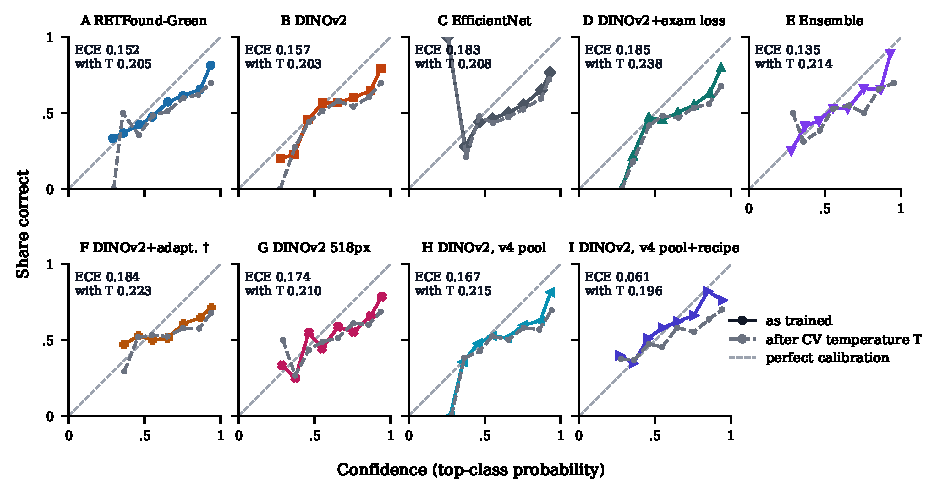
\includegraphics[width=\textwidth]{fig_reliability_dev_eye.pdf}
\caption{Reliability of the eye-level top-class probability at the unseen hospital (dev half), ten equal-width bins, seeds pooled: as trained (colour) and after each seed's CV temperature $T$ (grey). $^\dagger$Transductive.}
\label{fig:reliability}
\end{figure*}

\begin{figure*}[!t]
\centering
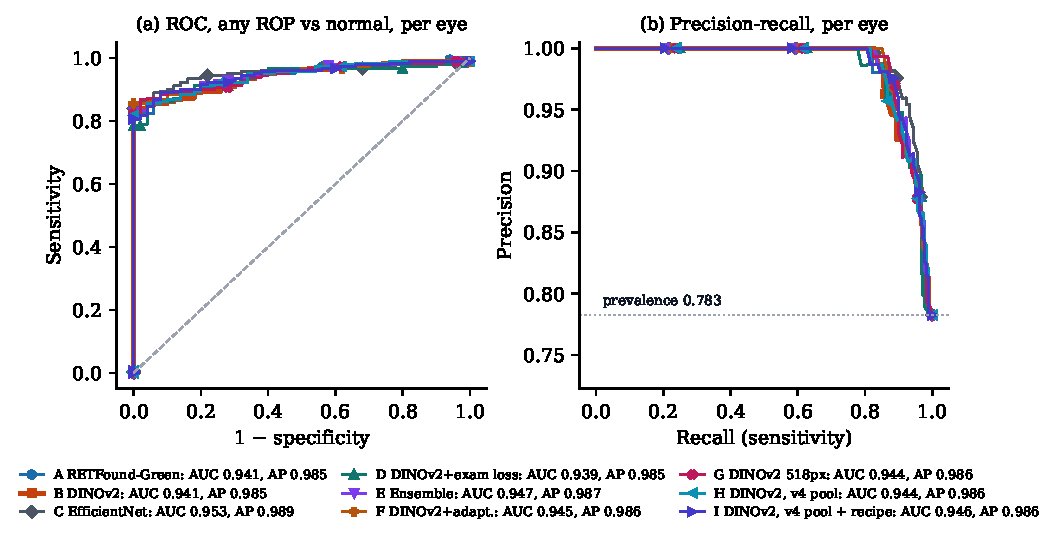
\includegraphics[width=\textwidth]{fig_roc_pr_dev_eye.pdf}
\caption{Any ROP vs normal per eye at the unseen hospital (dev half), all arms. Curves use the eye score averaged over each arm's \devLists{} models, so their AUC and AP (legend) differ slightly from Table~\ref{tab:headline}, which averages per-model values. Dotted: prevalence.}
\label{fig:rocpr}
\end{figure*}

\begin{table*}[!t]
\caption{Recipe and cost. Shared by every trained arm: circle-crop, letterbox, CLAHE; class-balanced cross-entropy~\cite{cui2019}; strong and site-randomising augmentation; batch 16; AdamW; one-cycle cosine schedule; last-epoch weights. LLRD: layer-wise lr decay; LS: label smoothing. F's adaptation is self-ensembling~\cite{french2018}. Cost: mean over CV folds 0--4 and both seeds on Kaggle \gpu{} GPUs (kernel logs); C and E were not trained in this generation.}
\label{tab:recipe}
\centering\scriptsize\setlength{\tabcolsep}{3pt}
\begin{tabular}{@{}llcllcccc>{\raggedright\arraybackslash}p{6.2cm}cc@{}}
\toprule
Arm & Backbone & px & Norm. & Pool & Peak lr & LLRD & LS & Ep. & Differences from B's recipe & min/fold & img/s\\
\midrule
A & \texttt{retfound\_green} & 392 & half & v3 & 2e-4 & 0.8 & 0.05 & 20 & RETFound-Green weights & 32.1 & 38.6 \\
\textbf{B} & \texttt{dinov2\_s} & 392 & imagenet & v3 & 1e-4 & 0.8 & 0.05 & 20 & reference recipe & 33.3 & 31.9 \\
C & \texttt{effnetv2s} & 384 & imagenet & v3 & 3e-4 & -- & 0.05 & 20 & v2 flat softmax, natural sampler; saved predictions re-scored & -- & -- \\
D & \texttt{dinov2\_s} & 392 & imagenet & v3 & 1e-4 & 0.8 & 0.05 & 20 & LSE bag loss on Ostrava sessions, $K{=}8$, $\tau{=}1$ & 32.5 & 29.0 \\
E & -- & -- & -- & v3 & -- & -- & -- & -- & mean of A, B, C probabilities, matched by seed; no training & -- & -- \\
F$^\dagger$ & \texttt{dinov2\_s} & 392 & imagenet & v3 & 1e-4 & 0.8 & 0.05 & 20 & self-ensembling on unlabelled dev photos, EMA 0.99, conf.\ $\ge$0.9 & 61.7 & 14.2 \\
G & \texttt{dinov2\_s} & 518 & imagenet & v3 & 1e-4 & 0.8 & 0.05 & 20 & 518 px & 58.1 & 19.2 \\
H & \texttt{dinov2\_s} & 392 & imagenet & v4 & 1e-4 & 0.8 & 0.05 & 20 & v4 pool (per-device quality filter) & 34.1 & 31.2 \\
I & \texttt{dinov2\_s} & 392 & imagenet & v4 & 1e-4 & 0.8 & 0.1 & 20 & EMA weights 0.999; 1 head-only epoch; label smoothing 0.1; rot.\ $\pm$180$^\circ$, crop $\ge$0.85, gamma, noise, Fourier swap $p\,0.5$ & 34.8 & 32.1 \\
\bottomrule
\end{tabular}

\end{table*}

\begin{figure*}[!t]
\centering
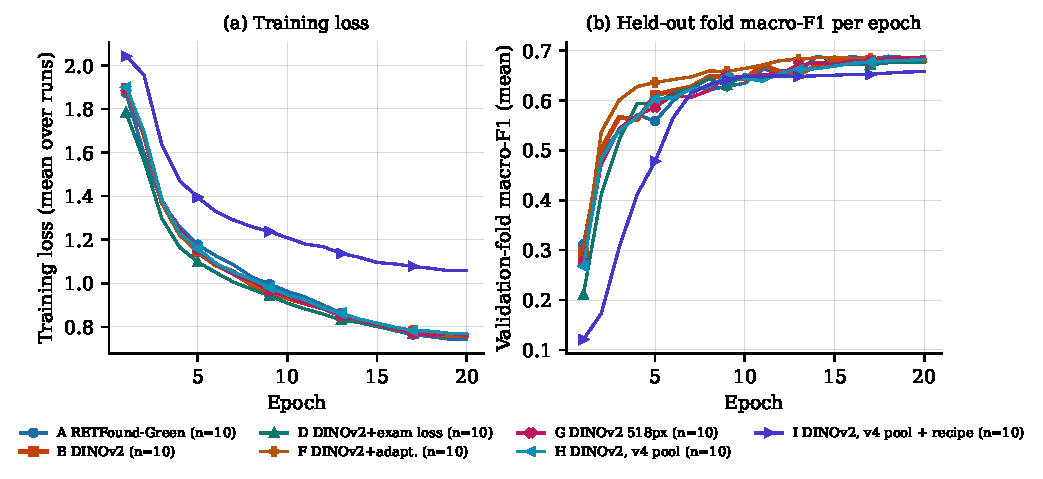
\includegraphics[width=\textwidth]{fig_training_curves.pdf}
\caption{Training curves, mean over each arm's \nRuns{} runs (five CV folds $\times$ two seeds): (a) training loss; (b) macro-F1 on the held-out fold per epoch. I's loss sits higher by construction (its label smoothing, Table~\ref{tab:recipe}) and its F1 is measured on EMA weights. C and E have no curves.}
\label{fig:training}
\end{figure*}

\begin{table*}[!t]
\caption{Secondary readouts. Dev per photograph: QWK5 with 95\% CI, no eye aggregation. CV per cohort at its label unit: Ostrava examination session, ROP-VL eye examination, Shenzhen photograph~\cite{nagpure2026}. Ordinal decoder (Amendment~3b): expected stage cut by four thresholds fitted on CV only; argmax remains primary.}
\label{tab:secondary}
\centering\scriptsize\setlength{\tabcolsep}{5pt}
\begin{tabular}{@{}ll@{\hspace{6pt}}ccc@{\hspace{6pt}}cc@{}}
\toprule
 & Dev half & \multicolumn{3}{c}{CV, each cohort at its label unit} & \multicolumn{2}{c}{Ordinal decoder}\\
\cmidrule(lr){3-5}\cmidrule(l){6-7}
Arm & per photo QWK5 [95\% CI] & Ostrava exam & ROP-VL eye-exam & Shenzhen photo & CV & Dev eye\\
\midrule
A & 0.407 [0.336, 0.478] & 0.679 & 0.931 & 0.969 & 0.757 & 0.761 \\
\textbf{B} & 0.416 [0.342, 0.488] & 0.701 & 0.930 & 0.967 & 0.788 & 0.760 \\
C & 0.438 [0.362, 0.510] & 0.775 & 0.921 & 0.967 & 0.815 & 0.771 \\
D & 0.412 [0.339, 0.484] & 0.846 & 0.925 & 0.967 & 0.808 & 0.762 \\
E & 0.418 [0.346, 0.492] & 0.769 & 0.940 & 0.971 & 0.812 & 0.776 \\
F$^\dagger$ & 0.416 [0.342, 0.490] & 0.693 & 0.935 & 0.967 & 0.783 & 0.748 \\
G & 0.413 [0.343, 0.487] & 0.695 & 0.925 & 0.967 & 0.779 & 0.764 \\
H & 0.412 [0.338, 0.486] & 0.710 & 0.933 & 0.968 & 0.789 & 0.762 \\
I & 0.441 [0.363, 0.519] & 0.712 & 0.933 & 0.962 & 0.807 & 0.777 \\
\bottomrule
\end{tabular}

\end{table*}

\clearpage
\section{Earlier Generations (Historical)}\label{sec:hist}
Each table keeps its own protocol and definitions; none is comparable with Tables~\ref{tab:headline}--\ref{tab:secondary} without its caveat. Glaucoma and diabetic-retinopathy models (\path{MODEL_HISTORY.md}) are outside this ROP compendium.

\begin{table}[!t]
\caption{v1 (June 2026): EfficientNet-B3, one shared model for binary ROP and DR. P / R: precision / recall. \emph{Caveat}: image-level split and two diseases in one model; retired.}
\label{tab:v1}
\centering\scriptsize\setlength{\tabcolsep}{2.0pt}
\begin{tabular}{@{}>{\raggedright\arraybackslash}p{1.45cm}rccccc@{}}
\toprule
Split & n & Acc. & mF1 & No ROP P / R & ROP P / R & ROP F1\\
\midrule
ROP val & 928 & 0.647 & 0.646 & 0.476 / 0.933 & 0.941 / 0.510 & 0.661 \\
ROP test & 1{,}502 & 0.733 & 0.731 & 0.644 / 0.913 & 0.891 / 0.585 & 0.706 \\
DR val, ep.\ 5 & -- & 0.719 & 0.497 & -- & -- & -- \\
\bottomrule
\end{tabular}

\end{table}

\begin{table}[!t]
\caption{June 2026 binary sweep (ROP yes/no, Ostrava, sweep validation split; QWK$_2$ binary kappa), and, $^\ast$, a separate ResNet50 run on its own validation and test split (\texttt{results/rop/metrics.json}). \emph{Caveat}: inflated by a device shortcut (image dimensions alone predicted ROP with AUC \shortcutAUC{}).}
\label{tab:sweep}
\centering\scriptsize\setlength{\tabcolsep}{2.2pt}
\begin{tabular}{@{}lcccccc@{}}
\toprule
Architecture & Acc. & mF1 & QWK$_2$ & AUC & Params (M) & CPU ms\\
\midrule
efficientnet\_b0 & 0.758 & 0.757 & 0.525 & 0.867 & 4.01 & 56.2 \\
efficientnet\_v2\_s & 0.706 & 0.701 & 0.431 & 0.870 & 20.18 & 130.1 \\
mobilenet\_v3\_large & 0.744 & 0.743 & 0.500 & 0.857 & 4.2 & 34.4 \\
resnet50 & 0.886 & 0.882 & 0.766 & 0.964 & 23.51 & 157.2 \\
densenet121 & 0.764 & 0.764 & 0.537 & 0.887 & 6.96 & 136 \\
\midrule
resnet50$^\ast$ val & 0.747 & 0.740 & 0.499 & 0.842 & -- & -- \\
resnet50$^\ast$ test & 0.844 & 0.843 & 0.688 & 0.927 & -- & -- \\
\bottomrule
\end{tabular}

\end{table}

\begin{table*}[!t]
\caption{v2 (August 2026): EfficientNetV2-S structured head (CORN ordinal + AP-ROP branch + site adversary, \vtStructParams{} parameters) vs flat softmax, natural sampling, five-fold CV. QWK$_6$: legacy six-class definition; QWK5$_d$: v2's ``corrected'' definition, rows with true or predicted AP-ROP removed (optimistic); QWK5: the v3 definition used in Table~\ref{tab:headline}. Dev and locked: unseen hospital; eye = max over views; locked half opened once (\lockedOpened{}); dev and locked values are means over the five fold checkpoints. The served fold-0 checkpoint (structured, seed \seedA{}) scored per photograph QWK5$_d$ \vtServedImgQ{}, accuracy \vtServedImgAcc{}, any-ROP AUC \vtServedImgAUC{}, and per eye QWK5$_d$ \vtServedEyeQ{} \vtServedEyeQci{}, accuracy \vtServedEyeAcc{}, mF1 \vtServedEyeMF{}. \emph{Caveat}: arm C re-scores the flat arm under v3 rules; v2's headline eye number was on the locked half, v3's on the dev half.}
\label{tab:v2}
\centering\scriptsize\setlength{\tabcolsep}{3.4pt}
\begin{tabular}{@{}ll@{\hspace{4pt}}cccccc@{\hspace{5pt}}c@{\hspace{5pt}}cc@{\hspace{5pt}}ccc@{}}
\toprule
 & & \multicolumn{6}{c}{CV pooled OOF, 6{,}700 photos} & Dev & \multicolumn{2}{c}{Locked, photo} & \multicolumn{3}{c}{Locked, eye (max)}\\
\cmidrule(lr){3-8}\cmidrule(lr){9-9}\cmidrule(lr){10-11}\cmidrule(l){12-14}
Head & Seed & QWK$_6$ & QWK5$_d$ & QWK5 & Acc. & mF1 & AUC & QWK5 & QWK5$_d$ & QWK5 & QWK5$_d$ & QWK5 & Acc.\\
\midrule
Structured & 42 & 0.761 & 0.897 & 0.807 & 0.786 & 0.652 & 0.969 & 0.755 & 0.473 & 0.517 & 0.813 & 0.823 & 0.646 \\
 & 1337 & 0.783 & 0.905 & 0.824 & 0.804 & 0.666 & 0.967 & 0.752 & 0.456 & 0.500 & 0.794 & 0.808 & 0.627 \\
Flat & 42 & 0.777 & 0.897 & 0.820 & 0.789 & 0.655 & 0.968 & 0.756 & 0.492 & 0.551 & 0.808 & 0.823 & 0.635 \\
 & 1337 & 0.770 & 0.898 & 0.813 & 0.787 & 0.658 & 0.966 & 0.764 & 0.486 & 0.543 & 0.801 & 0.818 & 0.630 \\
\bottomrule
\end{tabular}

\end{table*}

\begin{table}[!t]
\caption{v2 five-backbone staging sweep (flat softmax, six classes, fold~0 and the leave-site fold, seed \seedA{}). \emph{Caveat}: one fold and one seed; the in-fold spread lies inside one run's end-of-schedule noise; legacy QWK not recomputed.}
\label{tab:backbones}
\centering\scriptsize\setlength{\tabcolsep}{1.8pt}
\begin{tabular}{@{}lcccc@{}}
\toprule
Backbone & Params & mF1, fold 0 & mF1, site fold & AP-ROP recall\\
\midrule
EfficientNetV2-S & 20.2M & 0.520 & 0.641 & 0.183 \\
DeiT3-S & 21.8M & 0.517 & 0.507 & 0.174 \\
ConvNeXt-T (in12k) & 27.8M & 0.509 & 0.530 & 0.162 \\
CAFormer-S18 & 24.3M & 0.498 & 0.507 & 0.221 \\
EfficientNet-B0 & 4.0M & 0.492 & 0.536 & (pre-metric-fix) \\
\bottomrule
\end{tabular}

\end{table}

\begin{table}[!t]
\caption{Retired v2 structured arm trained with a class-balanced sampler, fold~0. \emph{Caveat}: fold~0 only, legacy six-class QWK; the CORN cascade calibrates to the training prevalence.}
\label{tab:sampler}
\centering\scriptsize\setlength{\tabcolsep}{3pt}
\begin{tabular}{@{}>{\raggedright\arraybackslash}p{2.7cm}ccc@{}}
\toprule
Fold 0 & Balanced sampler & Natural (v2) & Flat\\
\midrule
QWK (legacy 6-class, as reported at the time) & 0.121 & 0.569 & 0.594 \\
stage\_4\_5 precision & 0.043 & --- & --- \\
Normal recall & 0.456 & 0.939 & --- \\
macro-F1 & 0.403 & 0.553 & 0.563 \\
\bottomrule
\end{tabular}

\end{table}

\begin{table}[!t]
\caption{Retired ResNet50 binary screener: external audit at the unseen hospital (663 dev photographs). \emph{Caveat}: its threshold was set at another hospital; the v2 dev AUC is in-sample for v2's own threshold choice.}
\label{tab:screener}
\centering\scriptsize\setlength{\tabcolsep}{3pt}
\begin{tabular}{@{}>{\raggedright\arraybackslash}p{4.4cm}>{\raggedright\arraybackslash}p{3.9cm}@{}}
\toprule
External audit & Value\\
\midrule
images flagged positive & 663 of 663 --- including every healthy eye \\
specificity at the served threshold & 0.000 \\
external AUC & 0.691 \\
minimum score among external healthy eyes & 0.2939 \\
served threshold & 0.1933 \\
external dev AUC (``any ROP'') (retired / v2 structured) & 0.691 / 0.821 \\
external locked AUC (``any ROP'') (retired / v2 structured) & not measured / 0.835 \\
\bottomrule
\end{tabular}

\end{table}

\section{Independent Teammate Packages (Photo-Level Split, Four Classes)}\label{sec:mate}
Three packages trained by a team member on one Windows GPU (3--5 Nov 2026), outside the protocol, collected from their result files (\texttt{scripts/collect\_teammate\_packages.py}, \texttt{\mateCommit}); no model was re-run. \textbf{Data} (Table~\ref{tab:matedata}): \mateN{} photographs of this project (ROP-VL \mateSrcRopvl{}, Multi-View \mateSrcMultiview{}, Shenzhen \mateSrcShenzhen{}, \mateUnmatched{} renamed copies not matched by file name) in four classes (Normal, stage~1, 2, 3; no stage~4/5, no AP-ROP), split 80/10/10 \emph{by photograph} with seed \seedA{} (rop\_ml: 80/20), and the same preprocessing in all three (black-border crop, resize, CLAHE). \textbf{Why these numbers are not comparable with Tables~\ref{tab:headline}--\ref{tab:secondary}.} (i)~The split is by photograph: \mateLeakTest{} of the test photographs and \mateLeakVal{} of the validation photographs share an infant with the training set (\mateLeakMV{} of the Multi-View test photographs), so every test number is optimistic by an unmeasured amount. (ii)~\mateDevTrain{} development-half and \mateLockedTrain{} locked-half photographs were used for training, so none of these models can ever be scored on this project's test halves. (iii)~Four classes, \mateTest{} test photographs: a 95\% CI about $\pm$\mateHalfWidth{} points, wider than most differences between runs. (iv)~Early stopping and ensemble membership were chosen on \mateVal{} validation photographs.

\textbf{rop\_ml} (Table~\ref{tab:mateml}): \mateMLFeat{} hand-made features per 256-px photograph (colour statistics, LBP, GLCM, HOG, Frangi vessel responses), training rows balanced by augmentation, twelve learners ranked by five-fold CV accuracy; best \mateMLBest{}, test accuracy \mateMLAcc{}, QWK \mateMLQ{}. \textbf{rop\_cnn} (Table~\ref{tab:matecnn}): six ImageNet-pretrained timm CNNs at 224\,px, head warm-up then full fine-tuning, AdamW, cosine schedule, class-weighted cross-entropy with label smoothing, early stopping on validation macro-F1, three-view flip TTA; best \mateCNNBest{}, test accuracy \mateCNNAcc{}, QWK \mateCNNQ{}; \mateCNNDiverged{} diverged (\mateCNNDivergedAcc{}). \textbf{rop\_foundation} (Table~\ref{tab:matefm}): RETFound-DINOv2 ViT-L/14~\cite{zhou2023} kept frozen (\mateFMtotal{}\,M weights) with LoRA adapters~\cite{hu2022} of rank~16 on the attention and MLP projections of all 24 blocks and a linear head (\mateFMtrainable{}\,M trainable), bf16, 4-view flip TTA; a stage-2 sweep of one change each (10 epochs) chose the 280-px variant on validation, trained for 30 epochs with three seeds: test accuracy \mateFMlo{}--\mateFMhi{} (mean \mateFMmean{}, SD \mateFMsd{}), against \mateFMbaseAcc{} for the attention-only adapters (\mateFMbaseTrainable{}\,M) and \mateFMcomboAcc{} when four changes were combined. Averaging the three seeds gives \mateEnsAcc{} (QWK \mateEnsQ{}); adding the four CNNs gives the best number in the packages, \mateBestAcc{} \mateBestAccci{} (QWK \mateBestQ{}, AUC \mateBestAUC{}). Per-class recall and precision of the best models: Table~\ref{tab:matestage}; all \nMateSeries{} models with Wilson CIs: Fig.~\ref{fig:teammate}. \textbf{Reading.} Within the packages, a frozen retina-pretrained ViT-L with \mateFMtrainable{}\,M adapted weights ties fully fine-tuned CNNs, and seed-to-seed spread exceeds every single-change effect in the sweep; averaging models is the only reliable gain. The three-seed RETFound-DINOv2 ensemble is shown in the webapp beside B as a comparison only; B remains the selected model.

\begin{table*}[!t]
\caption{Teammate packages: their photo-level split against this project's splits, by file name (\mateMatched{} of \mateN{} matched). ``Elsewhere'': renamed copies not matched. Last column: validation/test photographs whose infant also has photographs in their training set (matched photographs only).}
\label{tab:matedata}
\centering\scriptsize\setlength{\tabcolsep}{4pt}
\begin{tabular}{@{}lr@{\hspace{6pt}}rrrr@{\hspace{6pt}}rrrr@{\hspace{6pt}}c@{}}
\toprule
 & & \multicolumn{4}{c}{Their classes} & \multicolumn{4}{c}{Where the photographs sit in this project} & Same infant\\
\cmidrule(lr){3-6}\cmidrule(lr){7-10}
Their split & Photos & N & S1 & S2 & S3 & CV pool & Dev half & Locked half & Elsewhere & as their training\\
\midrule
Train & 2{,}512 & 687 & 515 & 651 & 659 & 1{,}647 & 390 & 331 & 144 & -- \\
Val & 314 & 86 & 65 & 81 & 82 & 208 & 48 & 39 & 19 & 214 / 295 \\
Test & 315 & 86 & 64 & 82 & 83 & 213 & 50 & 38 & 14 & 221 / 301 \\
\bottomrule
\end{tabular}

\end{table*}

\begin{table}[!t]
\caption{rop\_ml: twelve classical learners on \mateMLFeat{} features; CV: five-fold accuracy on the (augmented) training rows, which ranked the learners and chose the top three for the two ensembles; s: training seconds. \emph{Caveat}: photo-level split (Section~\ref{sec:mate}).}
\label{tab:mateml}
\centering\scriptsize\setlength{\tabcolsep}{3pt}
\begin{tabular}{@{}lccccccr@{}}
\toprule
 & CV & \multicolumn{5}{c}{Test, 629 photographs} & \\
\cmidrule(lr){3-7}
Model & Acc. & Acc. & Bal.\,acc. & mF1 & QWK & AUC & s\\
\midrule
SVM (RBF) & 0.562 & 0.585 & 0.576 & 0.576 & 0.547 & 0.812 & 23 \\
Soft Voting (top-3) & 0.571 & 0.585 & 0.571 & 0.569 & 0.573 & 0.810 & 593 \\
Extra Trees & 0.542 & 0.574 & 0.561 & 0.555 & 0.502 & 0.790 & 6 \\
XGBoost & 0.562 & 0.568 & 0.554 & 0.552 & 0.535 & 0.804 & 130 \\
HistGradBoost & 0.566 & 0.568 & 0.552 & 0.550 & 0.551 & 0.807 & 459 \\
LightGBM & 0.567 & 0.566 & 0.555 & 0.555 & 0.563 & 0.810 & 39 \\
MLP & 0.534 & 0.558 & 0.547 & 0.549 & 0.531 & 0.795 & 13 \\
Stacking (top-3) & 0.567 & 0.556 & 0.543 & 0.541 & 0.556 & 0.807 & 2{,}107 \\
Random Forest & 0.540 & 0.555 & 0.540 & 0.532 & 0.500 & 0.786 & 9 \\
CatBoost & 0.547 & 0.522 & 0.511 & 0.508 & 0.458 & 0.784 & 33 \\
KNN & 0.518 & 0.501 & 0.493 & 0.489 & 0.403 & 0.736 & 5 \\
Logistic Reg. & 0.520 & 0.488 & 0.477 & 0.475 & 0.410 & 0.762 & 6 \\
\bottomrule
\end{tabular}

\end{table}

\begin{table}[!t]
\caption{rop\_cnn: ImageNet-pretrained CNNs (timm), 224\,px, up to 40 epochs with early stopping on validation macro-F1; the soft vote averages the three models with the highest validation macro-F1 (EfficientNet-B2, ResNet50, DenseNet121). \emph{Caveat}: photo-level split.}
\label{tab:matecnn}
\centering\scriptsize\setlength{\tabcolsep}{1.9pt}
\begin{tabular}{@{}lccc@{\hspace{6pt}}ccccc@{}}
\toprule
 & & & Val & \multicolumn{5}{c}{Test, 315 photographs}\\
\cmidrule(l){5-9}
Model & Par.\,(M) & Ep. & mF1 & Acc. & Bal. & mF1 & QWK & AUC\\
\midrule
resnest50d & 25.4 & 32 & 0.821 & 0.835 & 0.827 & 0.828 & 0.898 & 0.956 \\
densenet121 & 7.0 & 36 & 0.822 & 0.822 & 0.816 & 0.815 & 0.880 & 0.942 \\
efficientnet\_b2 & 7.7 & 40 & 0.832 & 0.819 & 0.812 & 0.811 & 0.884 & 0.943 \\
resnet50 & 23.5 & 40 & 0.827 & 0.810 & 0.802 & 0.800 & 0.860 & 0.951 \\
mobilenetv3\_large\_100 & 4.2 & 22 & 0.769 & 0.775 & 0.775 & 0.769 & 0.840 & 0.925 \\
convnext\_tiny & 27.8 & 13 & 0.491 & 0.530 & 0.546 & 0.520 & 0.497 & 0.821 \\
\midrule
Soft vote, top 3 & -- & -- & 0.856 & 0.825 & 0.821 & 0.818 & 0.881 & 0.959 \\
\bottomrule
\end{tabular}

\end{table}

\begin{table*}[!t]
\caption{rop\_foundation: RETFound-DINOv2 ViT-L/14 frozen, LoRA adapters (rank 16, alpha 32 unless stated) on attention and MLP layers, linear 4-class head; lr $4\times10^{-4}$ unless stated; batch $4\times4$; class-weighted cross-entropy, label smoothing 0.1; best epoch by validation macro-F1; 4-view flip TTA. Probes: 10 epochs, one change each. \emph{Caveat}: photo-level split; the chosen configuration was picked on validation and is not better than the attention-only run on test.}
\label{tab:matefm}
\centering\scriptsize\setlength{\tabcolsep}{3.4pt}
\begin{tabular}{@{}l>{\raggedright\arraybackslash}p{3.3cm}ccc@{\hspace{5pt}}c@{\hspace{6pt}}ccccc@{}}
\toprule
 & & Trainable & & & Val & \multicolumn{5}{c}{Test, 315 photographs}\\
\cmidrule(l){7-11}
Run & Change & (M) & px & Epochs & mF1 & Acc. & Bal.\,acc. & mF1 & QWK & AUC\\
\midrule
\multicolumn{11}{@{}l}{\emph{Stage-2 probes, 10 epochs, seed 42 (one change each vs the first row)}}\\
p mlp & LoRA on attention + MLP (probe base) & 6.30 & 224 & 10 & 0.810 & 0.797 & 0.798 & 0.792 & 0.862 & 0.947 \\
p mlp r32 & rank 32, alpha 64 & 12.59 & 224 & 10 & 0.819 & 0.816 & 0.811 & 0.810 & 0.867 & 0.950 \\
p mlp dp1 & drop-path 0.1 & 6.30 & 224 & 10 & 0.830 & 0.797 & 0.799 & 0.793 & 0.861 & 0.951 \\
p mlp lr6e4 & lr 6e-4 & 6.30 & 224 & 10 & 0.829 & 0.829 & 0.825 & 0.823 & 0.897 & 0.958 \\
p mlp img280 & 280 px input & 6.30 & 280 & 10 & 0.834 & 0.822 & 0.821 & 0.818 & 0.875 & 0.959 \\
p mlp ord & ordinal auxiliary loss 0.3 & 6.30 & 224 & 10 & 0.807 & 0.806 & 0.807 & 0.803 & 0.876 & 0.951 \\
p mlp combo & r32 + dp 0.1 + lr 6e-4 + 280 px & 12.59 & 280 & 10 & 0.623 & 0.651 & 0.662 & 0.617 & 0.761 & 0.900 \\
\midrule
\multicolumn{11}{@{}l}{\emph{Full-length runs, 30 epochs max}}\\
final base s42 & attention-only LoRA, 30 ep & 2.37 & 224 & 30 & 0.817 & 0.825 & 0.818 & 0.818 & 0.900 & 0.956 \\
final mlp s42 & attention + MLP, 224 px, 30 ep & 6.30 & 224 & 25 & 0.816 & 0.778 & 0.763 & 0.765 & 0.860 & 0.948 \\
final mlp img280 s42 & chosen config, seed 42 & 6.30 & 280 & 25 & 0.846 & 0.787 & 0.787 & 0.779 & 0.870 & 0.950 \\
final mlp img280 s1 & chosen config, seed 1 & 6.30 & 280 & 30 & 0.841 & 0.822 & 0.818 & 0.815 & 0.888 & 0.952 \\
final mlp img280 s2 & chosen config, seed 2 & 6.30 & 280 & 30 & 0.846 & 0.832 & 0.827 & 0.826 & 0.889 & 0.951 \\
\midrule
3 seeds averaged & chosen config, seeds 42, 1, 2 & -- & -- & -- & 0.839 & 0.844 & 0.842 & 0.839 & 0.900 & 0.964 \\
3 seeds + 4 CNNs & plus EffNet-B2, ResNet50, DenseNet121, ResNeSt-50d & -- & -- & -- & 0.863 & 0.860 & 0.859 & 0.855 & 0.908 & 0.972 \\
\bottomrule
\end{tabular}

\end{table*}

\begin{table}[!t]
\caption{Recall / precision per class of the packages' best models on their own test photographs. \emph{Caveat}: photo-level split; rop\_ml's test set differs from the other two.}
\label{tab:matestage}
\centering\scriptsize\setlength{\tabcolsep}{2pt}
\begin{tabular}{@{}lcccc@{}}
\toprule
Model & Normal & Stage 1 & Stage 2 & Stage 3\\
\midrule
\multicolumn{5}{@{}l}{\emph{rop\_ml test, 629 photographs; n: Normal 172, S1 129, S2 163, S3 165}}\\
SVM (RBF) & 0.767 / 0.706 & 0.450 / 0.423 & 0.515 / 0.486 & 0.503 / 0.629 \\
\midrule
\multicolumn{5}{@{}l}{\emph{rop\_cnn and rop\_foundation test, 315 photographs; n: Normal 86, S1 64, S2 82, S3 83}}\\
resnest50d & 0.977 / 0.966 & 0.719 / 0.742 & 0.793 / 0.730 & 0.819 / 0.883 \\
CNN vote, top 3 & 1.000 / 0.915 & 0.781 / 0.676 & 0.720 / 0.756 & 0.783 / 0.942 \\
RETFound LoRA, 3 seeds & 0.965 / 0.965 & 0.828 / 0.726 & 0.707 / 0.806 & 0.868 / 0.857 \\
3 seeds + 4 CNNs & 0.988 / 0.966 & 0.859 / 0.733 & 0.744 / 0.803 & 0.843 / 0.921 \\
\bottomrule
\end{tabular}

\end{table}

\begin{figure}[!t]
\centering
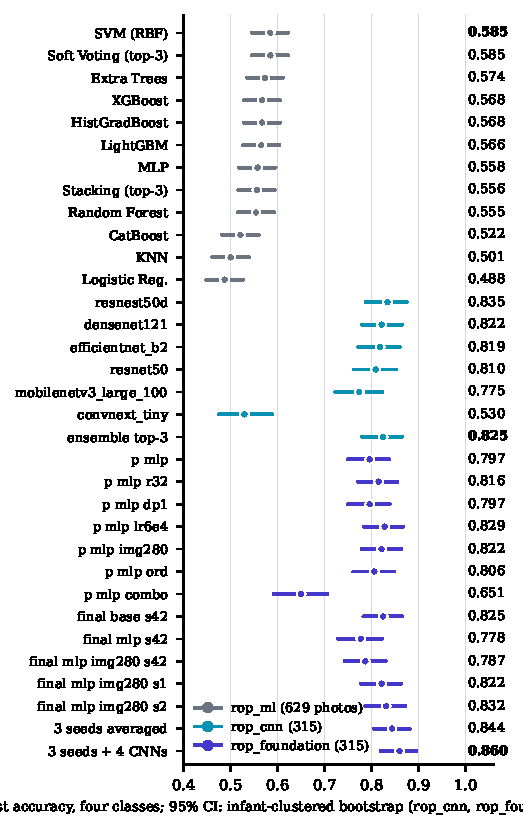
\includegraphics[width=\columnwidth]{fig_teammate.pdf}
\caption{Teammate packages: four-class test accuracy of every model with 95\% Wilson CI (n in the legend), one colour per package. Dotted: chance. Not comparable with Figs.~\ref{fig:selection}--\ref{fig:dev} (Section~\ref{sec:mate}).}
\label{fig:teammate}
\end{figure}

\clearpage
\section{Data}
Ostrava~\cite{timkovic2024} labels one examination session; ROP-VL one photograph with an eye-examination identifier; Shenzhen one photograph; Multi-View one eye.

\begin{table*}[!t]
\caption{Data by hospital and class. CV pool: every photograph lies in exactly one validation fold. Training-eligible: after per-infant caps (training sides only); the v4 pool adds a per-device Ostrava quality filter. $^\ast$Locked-half labels were not read; counts from the protocol.}
\label{tab:pool}
\centering\scriptsize\setlength{\tabcolsep}{4pt}
\begin{tabular}{@{}llrrrrrrrr@{}}
\toprule
Set & Unit & Normal & Stage 1 & Stage 2 & Stage 3 & Stage 4/5 & AP-ROP & Total & Infants\\
\midrule
\multicolumn{10}{@{}l}{\emph{Cross-validation pool (every photo is in exactly one validation fold)}}\\
Ostrava & photos & 2{,}980 & 252 & 458 & 125 & 0 & 470 & 4{,}285 & 148 \\
ROP-VL & photos & 623 & 236 & 338 & 241 & 89 & 148 & 1{,}675 & 983 \\
Shenzhen & photos & 234 & 89 & 163 & 254 & 0 & 0 & 740 & 397 \\
Total & photos & 3{,}837 & 577 & 959 & 620 & 89 & 618 & 6{,}700 & 1{,}528 \\
\midrule
\multicolumn{10}{@{}l}{\emph{Training-eligible after per-infant caps, v3 pool (arms A--G)}}\\
Ostrava & photos & 270 & 190 & 195 & 40 & 0 & 20 & 715 &  \\
ROP-VL & photos & 623 & 236 & 338 & 241 & 89 & 148 & 1{,}675 &  \\
Shenzhen & photos & 216 & 89 & 163 & 254 & 0 & 0 & 722 &  \\
Total & photos & 1{,}109 & 515 & 696 & 535 & 89 & 168 & 3{,}112 &  \\
\midrule
\multicolumn{10}{@{}l}{\emph{Training-eligible, v4 pool (arms H, I)}}\\
Ostrava & photos & 270 & 173 & 191 & 40 & 0 & 20 & 694 &  \\
ROP-VL & photos & 623 & 236 & 338 & 241 & 89 & 148 & 1{,}675 &  \\
Shenzhen & photos & 216 & 88 & 158 & 252 & 0 & 0 & 714 &  \\
Total & photos & 1{,}109 & 497 & 687 & 533 & 89 & 168 & 3{,}083 &  \\
\midrule
\multicolumn{10}{@{}l}{\emph{Unseen hospital (Multi-View), never in any fold}}\\
Dev half & photos & 150 & 190 & 135 & 168 & 14 & 6 & 663 & 116 \\
Dev half & eyes & 50 & 68 & 46 & 59 & 5 & 2 & 230 & 116 \\
Locked half$^\ast$ & photos & -- & -- & -- & -- & -- & -- & 661 & 116 \\
Locked half$^\ast$ & eyes & -- & -- & -- & -- & -- & -- & 230 & 116 \\
\bottomrule
\end{tabular}

\end{table*}

\begin{table*}[!t]
\caption{LOSO fold compositions: held-out source (test photographs after duplicate exclusion, infants) and training photographs by class in the v3 pool (A, B, D) and the v4 pool (H, I).}
\label{tab:losofolds}
\centering\scriptsize\setlength{\tabcolsep}{4pt}
\begin{tabular}{@{}llrrlrrrrrrr@{}}
\toprule
 & & & & & \multicolumn{7}{c}{Training photographs}\\
\cmidrule(l){6-12}
Held out & Fold file & Test photos & Infants & Pool & Normal & S1 & S2 & S3 & S4/5 & AP & Total\\
\midrule
Shenzhen & fold\_site.csv & 728 & 396 & v3 & 893 & 426 & 533 & 280 & 89 & 167 & 2{,}388 \\
 &  &  &  & v4 & 893 & 409 & 529 & 280 & 89 & 167 & 2{,}367 \\
Ostrava & fold\_loso\_ostrava.csv & 4{,}285 & 148 & v3 & 839 & 322 & 494 & 492 & 89 & 147 & 2{,}383 \\
 &  &  &  & v4 & 839 & 322 & 494 & 492 & 89 & 147 & 2{,}383 \\
ROP-VL & fold\_loso\_ropvl.csv & 1{,}673 & 983 & v3 & 486 & 276 & 351 & 292 & 0 & 20 & 1{,}425 \\
 &  &  &  & v4 & 486 & 259 & 347 & 292 & 0 & 20 & 1{,}404 \\
\bottomrule
\end{tabular}

\end{table*}

\section{Reproducibility}
Figures, tables and every number above: \texttt{.venv/bin/python scripts/paper3\_figures.py}, then \texttt{tectonic -X compile paper3\_results.tex}. No model is run and no file named \texttt{test\_locked} is read. PKG = \path{FINAL_MODEL_EVIDENCE_PACKAGE}.

\begin{table*}[!t]
\caption{Sources: path and last commit touching it (\texttt{git log}); ``git-ignored, on disk'' files exist only in the working tree (the CSVs fall under the repository's \texttt{*.csv} rule).}
\label{tab:repro}
\centering\scriptsize\setlength{\tabcolsep}{4pt}
\begin{tabular}{@{}>{\raggedright\arraybackslash}p{4.6cm}>{\raggedright\arraybackslash}p{9.6cm}l@{}}
\toprule
Item & Path & Commit\\
\midrule
Protocol and amendments (first commit) & \texttt{docs/\allowbreak{}paper/\allowbreak{}PROTOCOL\_V2.md} & \texttt{ac33f29} 2026-10-20 \\
Protocol, latest amendment & \texttt{docs/\allowbreak{}paper/\allowbreak{}PROTOCOL\_V2.md} & \texttt{0e55915} 2026-10-31 \\
Scores, arms A--I (selection, LOSO, contrasts) & \texttt{results/\allowbreak{}rop/\allowbreak{}v3/\allowbreak{}v3\_scores.json} & \texttt{b827cce} 2026-11-01 \\
Per-arm report data (tables, curves) & \texttt{results/\allowbreak{}rop/\allowbreak{}v3/\allowbreak{}report\_data.json} & \texttt{b827cce} 2026-11-01 \\
v4 pool summary & \texttt{results/\allowbreak{}prepared/\allowbreak{}rop\_staging/\allowbreak{}v4/\allowbreak{}v4\_summary.json} & \texttt{1efccd0} 2026-10-31 \\
Scorer & \texttt{scripts/\allowbreak{}rop\_v3\_score.py} & \texttt{2bbc55a} 2026-10-31 \\
Report-data builder & \texttt{scripts/\allowbreak{}rop\_v3\_report\_data.py} & \texttt{d8b7ec1} 2026-10-31 \\
v4 model report & \texttt{scripts/\allowbreak{}rop\_v4\_model\_report.py} & \texttt{3f7b79f} 2026-11-01 \\
This paper's figures and tables & \texttt{scripts/\allowbreak{}paper3\_figures.py} & not yet committed \\
Model chronology & \texttt{docs/\allowbreak{}paper/\allowbreak{}MODEL\_HISTORY.md} & \texttt{11b8f5e} 2026-10-31 \\
v2 QWK recalculation (3 definitions) & \texttt{PKG/\allowbreak{}20\_AUDIT/\allowbreak{}verification\_pass\_2/\allowbreak{}06\_VALIDATION/\allowbreak{}qwk\_5class\_vs\_6class\_recalculation.csv} & git-ignored, on disk \\
v2 CV summary & \texttt{PKG/\allowbreak{}07\_TEST\_RESULTS/\allowbreak{}metrics\_summary.csv} & git-ignored, on disk \\
v2 locked, served checkpoint (eye CIs) & \texttt{PKG/\allowbreak{}08\_EYE\_LEVEL\_ANALYSIS/\allowbreak{}eye\_confidence\_intervals.csv} & git-ignored, on disk \\
Five-backbone sweep & \texttt{PKG/\allowbreak{}19\_COMPARISONS/\allowbreak{}retired\_models/\allowbreak{}five\_backbone\_benchmark.md} & \texttt{aaffcf0} 2026-09-22 \\
Weighted-sampler arm & \texttt{PKG/\allowbreak{}19\_COMPARISONS/\allowbreak{}retired\_models/\allowbreak{}weighted\_sampler\_v1\_arm.md} & \texttt{aaffcf0} 2026-09-22 \\
ResNet50 screener audit & \texttt{PKG/\allowbreak{}19\_COMPARISONS/\allowbreak{}retired\_models/\allowbreak{}resnet50\_binary\_screener.md} & \texttt{aaffcf0} 2026-09-22 \\
June 2026 binary sweep & \texttt{results/\allowbreak{}sweep\_rop.md} & \texttt{2bb8db3} 2026-06-28 \\
ResNet50 val/test metrics & \texttt{results/\allowbreak{}rop/\allowbreak{}metrics.json} & \texttt{c042d7f} 2026-07-31 \\
v1 EfficientNet-B3 evaluation & \texttt{junk/\allowbreak{}unified\_model/\allowbreak{}evaluation\_unified.txt} & git-ignored, on disk \\
Arm configs (A, B, D, F--I; C) & \texttt{configs/\allowbreak{}rop\_staging\_*.yaml} & \texttt{9c9ab65} 2026-10-31 \\
\bottomrule
\end{tabular}

\end{table*}

\section*{Compliance with Ethical Standards}
This retrospective study used only publicly released, de-identified datasets under their licences (Ostrava/RIDIRP, ROP-VL, Shenzhen, Multi-View ROP, CC BY-NC); no new data were collected and no ethical approval was required. RETFound-Green's and RETFound-DINOv2's weights are used under their non-commercial licences. The system is research software and not a medical device. No funding was received; the authors declare no conflicts of interest.

\section*{Acknowledgments}
We thank the releasing institutions and Kaggle for the free GPU time on which every model was trained. \FILL{venue-specific AI disclosure, e.g.: Claude (Anthropic) was used to draft and edit code and text in all sections under the authors' direction; the authors verified every number against the committed result files and take full responsibility for the content.}

\begin{thebibliography}{99}
\bibitem{icrop3} M.~F.~Chiang, G.~E.~Quinn, A.~R.~Fielder, \emph{et al.}, ``International classification of retinopathy of prematurity, third edition,'' \emph{Ophthalmology}, vol.~128, no.~10, pp.~e51--e68, 2021.
\bibitem{engelmann2025} J.~Engelmann, \emph{et al.}, ``RETFound-Green: a green retinal foundation model,'' \emph{Nat. Commun.}, 2025. \FILL{confirm title, volume, article number}
\bibitem{oquab2024} M.~Oquab, T.~Darcet, T.~Moutakanni, \emph{et al.}, ``DINOv2: learning robust visual features without supervision,'' \emph{Trans. Mach. Learn. Res.}, 2024.
\bibitem{tan2021} M.~Tan and Q.~V.~Le, ``EfficientNetV2: smaller models and faster training,'' in \emph{Proc. ICML}, 2021, pp.~10096--10106.
\bibitem{nagpure2026} P.~Nagpure, R.~Bait, P.~Rangnekar, Y.~Shengale, and A.~Kumar, ``What the label unit hides: an audited multi-hospital benchmark for ICROP retinopathy of prematurity staging,'' \FILL{preprint venue, DOI, 2026}.
\bibitem{cui2019} Y.~Cui, M.~Jia, T.-Y.~Lin, Y.~Song, and S.~Belongie, ``Class-balanced loss based on effective number of samples,'' in \emph{Proc. IEEE/CVF CVPR}, 2019, pp.~9268--9277.
\bibitem{french2018} G.~French, M.~Mackiewicz, and M.~Fisher, ``Self-ensembling for visual domain adaptation,'' in \emph{Proc. ICLR}, 2018.
\bibitem{zhou2023} Y.~Zhou, M.~A.~Chia, S.~K.~Wagner, \emph{et al.}, ``A foundation model for generalizable disease detection from retinal images,'' \emph{Nature}, vol.~622, pp.~156--163, 2023.
\bibitem{hu2022} E.~J.~Hu, Y.~Shen, P.~Wallis, \emph{et al.}, ``LoRA: low-rank adaptation of large language models,'' in \emph{Proc. ICLR}, 2022.
\bibitem{timkovic2024} J.~Timkovi\v{c}, \emph{et al.}, ``Retinal image dataset of infants and retinopathy of prematurity,'' \emph{Sci. Data}, vol.~11, art.~814, 2024.
\end{thebibliography}
\end{document}
